\hypertarget{c6}{\chapter{Organisation du projet}}

\section{Méthodes de travail}

Cette année, nous avons décidé d’utiliser une méthode de travail suivant un cycle en V.
Cette méthode nous semble la plus adaptée pour notre cas. En effet, les limites du projet
sont clairement définies, de même que le cahier des charges et les spécifications générales.
Ainsi, durant la première phase du projet, au premier semestre, nous allons mettre en place
des réunions régulières pour bien évaluer le travail à réaliser. Durant la seconde phase,
au second semestre, nous effectuerons des réunions pour voir l’avancée de la programmation.

\paragraph{}
Comme le projet peut facilement être découpé en 4 parties (Préparation des données,
Base de données, IHM et Gestion du reconnaisseur), nous avons décidé de diviser notre
groupe en 4 pour pouvoir faire avancer le projet en parallèle. Nous estimons qu’il est
tout de même important de garder une forte communication et cohésion entre les différents
groupes, donc nous avons mis en place différents systèmes de communication. Pour gérer
l’organisation, nous utiliserons Trello et Microsoft Project. Pour le partage de fichiers,
notamment pour la rédaction des rapports, nous utiliserons Google Drive et Git.
Pour la gestion du code, nous utiliserons aussi Git. Enfin, pour communiquer, nous
utiliserons une conversation Messenger (qui servira à transmettre des informations de
manière rapide), un groupe Facebook (qui servira à publier la répartition des tâches et
les objectifs de chaque semaine de manière fixe et accessible) et probablement des salons
Discord qui permettront à chaque groupe de communiquer sans perturber les autres groupes.

\paragraph{}
Pour l’instant, nous avons décidé d’établir des réunions hebdomadaires (voire deux réunions
par semaine en cas de retard ou de livrables à rendre). Cette planification sera probablement
modifiée au second semestre lors du début du développement, car le groupe sera réduit de
moitié à cause des départs en mobilité. En effet, à partir du mois de janvier et du début du
second semestre, certaines personnes partiront faire une mobilité à l’étranger et ne
travailleront donc plus sur le projet. Notre groupe sera amputé de trois personnes : Kevin
DESPOULAINS, Gaël GENDRON et Corentin GUILLOUX.

\paragraph{}
L’arrivée ou le départ de membres n’est pas rare dans le déroulement d’un projet et nous avons
réfléchi à une organisation qui permet de faire une transition souple entre le premier semestre
où nous sommes huit et le second où nous serons cinq. Les membres partant à l’étranger ne
travailleront en effet pas seuls sur une partie mais leur travail sera réparti sur plusieurs
aspects du projet où ils travailleront avec des personnes restant au second semestre. Cette
répartition est faite pour qu’au moment de leur départ, il y ait au moins une personne du groupe
restant sachant exactement ce qui a été fait par les étudiants qui sont partis.

\section{Répartition des tâches}

Afin de répondre aux besoins du projet, nous avons mis en place 3 rôles. Ces 3 rôles ne sont pas fixes,
ils peuvent être modifiés en cas de besoin. Le premier rôle est le chef de projet. Ce rôle n’est donc pas
assigné de manière fixe, il change régulièrement. Nous avons établi un calendrier précis qui donne l’indication
de qui est chef de projet à chaque instant. Voici les rotations prévues :

\paragraph{}
\begin{center}
\begin{tabular}{ | l | l | l | }
\hline
{\textbf{Chef de projet}}   &   {\textbf{Début}}    &   {\textbf{Fin}}  \\ \hline \rowcolor[RGB]{182, 215, 168}
{Kevin DESPOULAINS}         &   {17/09/2018}        &	{07/10/2018}    \\ \hline \rowcolor[RGB]{255, 229, 153}
{Gaël GENDRON}              &   {08/10/2018}	    &	{28/10/2018}    \\ \hline \rowcolor[RGB]{249, 203, 156}
{Corentin GUILLOUX}         &   {05/11/2018}	    &	{30/11/2018}    \\ \hline \rowcolor[RGB]{234, 153, 153}
{Valentin FOUCHER}          &   {01/12/2018}	    &	{13/01/2019}    \\ \hline \rowcolor[RGB]{221, 126, 107}
{Enzo CRANCE}               &   {14/01/2019}	    &	{04/02/2019}    \\ \hline \rowcolor[RGB]{213, 166, 189}
{Charlotte RICHARD}         &   {05/02/2019}	    &	{10/03/2019}    \\ \hline \rowcolor[RGB]{180, 167, 214}
{Laure DU MESNILDOT}        &   {11/03/2019}	    &	{05/04/2019}    \\ \hline \rowcolor[RGB]{159, 197, 232}
{Timothée NEITTHOFFER}      &	{23/04/2019}	    &	{10/05/2019}    \\ \hline
\end{tabular}
\end{center}

\paragraph{}
\begin{mdframed}[frametitle={Figure 14 : Planning des rotations du rôle de chef de projet}, innerbottommargin=10]
\begin{center}
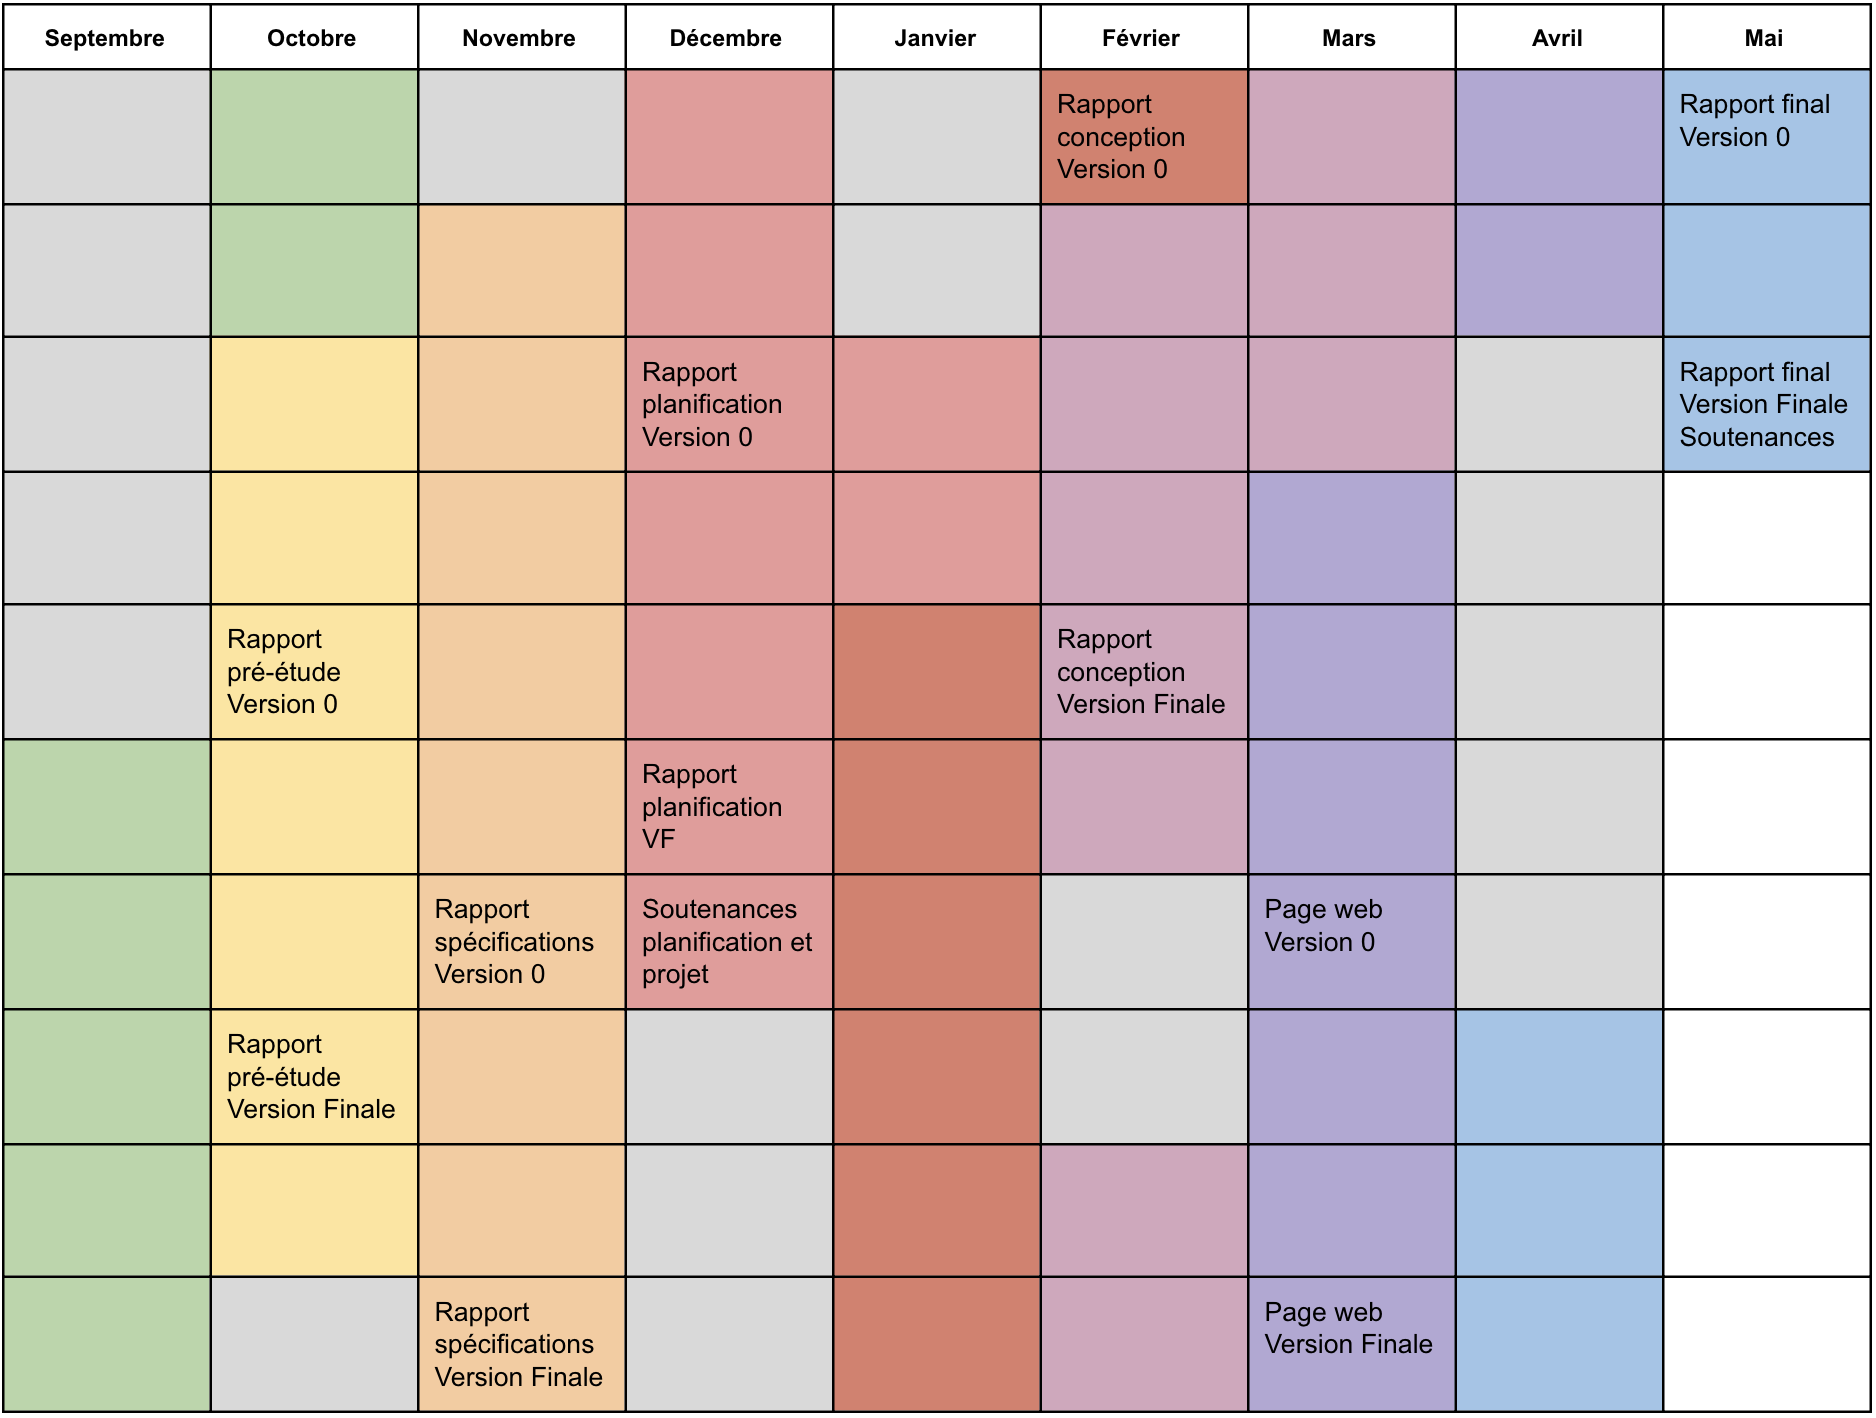
\includegraphics[width=\linewidth]{planning.png}
\end{center}
\end{mdframed}
    
\paragraph{}
Certaines périodes peuvent paraître plus longues pour certains que pour d’autres à cause des vacances
scolaires mais globalement chacun sera chef de projet durant 3 à 4 semaines. Le rôle du chef de projet est
avant tout de s’assurer du bon déroulement du projet. Il doit organiser les réunions, répartir équitablement
les tâches, surveiller les délais et diriger les réunions. Il doit également faire le lien avec les
différents intervenants et contrôler ce qui est écrit dans les rapports. Le deuxième rôle est celui de
responsable temps qui devra s’assurer que tout le groupe note bien le temps passé sur le projet en envoyant
des rappels réguliers. Il devra également gérer le temps de parole lors des réunions. Pour le moment,
c’est Timothée NEITTHOFFER qui a été désigné responsable temps. La personne jouant ce rôle peut être
modifiée sans problème au cours de l’année. Enfin, le dernier rôle est responsable qualité. Son but est de
contrôler la qualité du code réalisé. Au premier semestre c’est lui qui valide ou non les technologies que les
autres membres du groupe peuvent lui suggérer en les étudiant. Au second semestre il devra contrôler le code.
Pour le moment, c’est Enzo CRANCE qui a été désigné responsable qualité. Les autres membres du groupe travaillent
davantage sur les tâches que le chef de projet leur a confié comme la rédaction des rapports, la
recherche d’information, le développement, etc.

\section{Estimation de la planification des tâches}

Pour avoir une première estimation du planning, nous avons construit un diagramme de Gantt. L’explication est donnée en dessous.

\paragraph{}
\begin{mdframed}[frametitle={Figure 15 : Estimation de la planification des tâches}, innerbottommargin=10]
\begin{center}
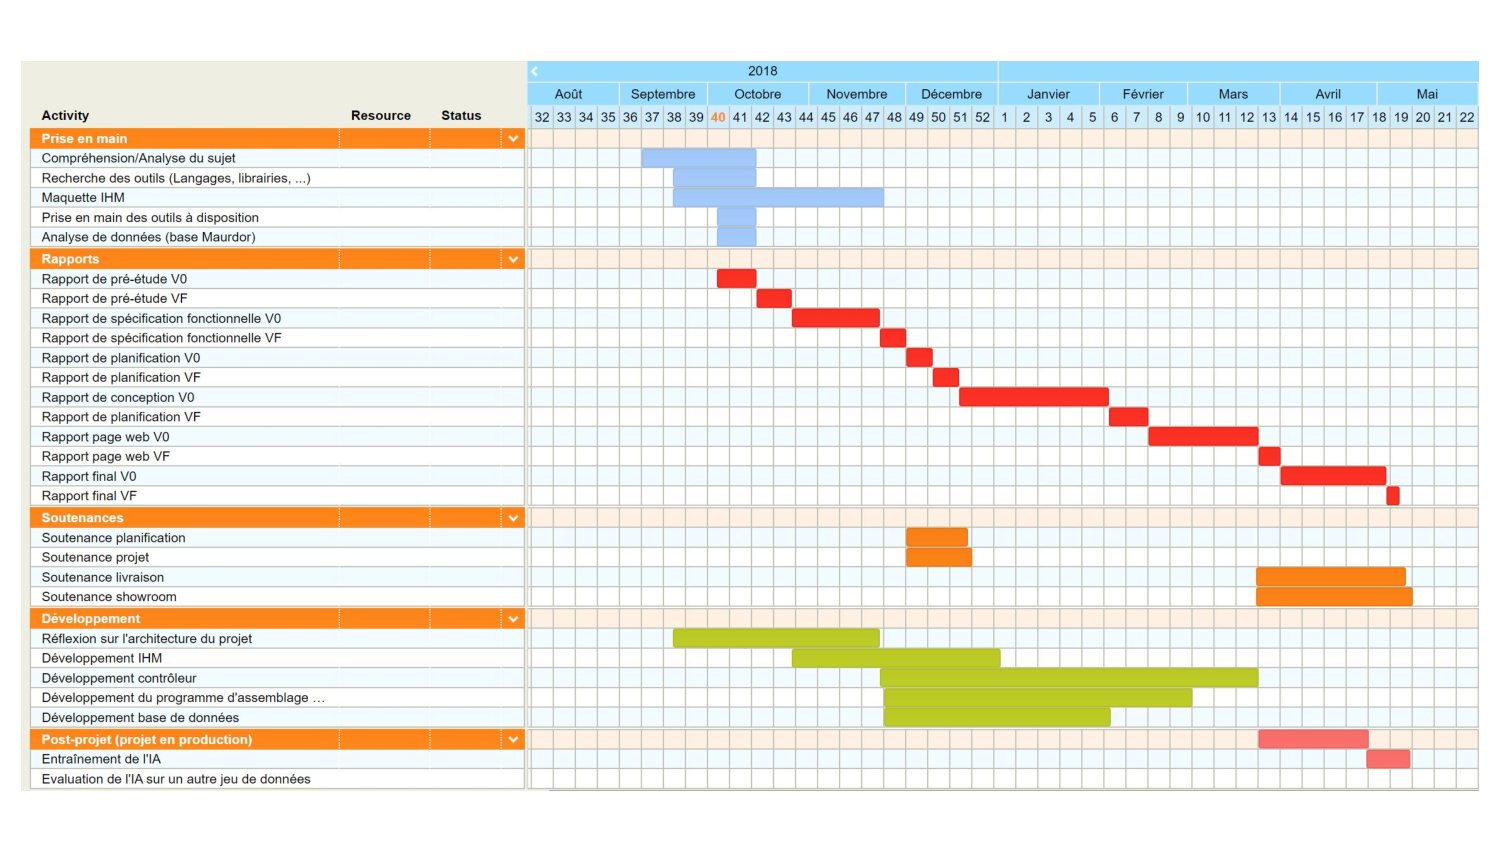
\includegraphics[width=\linewidth]{gantt.pdf}
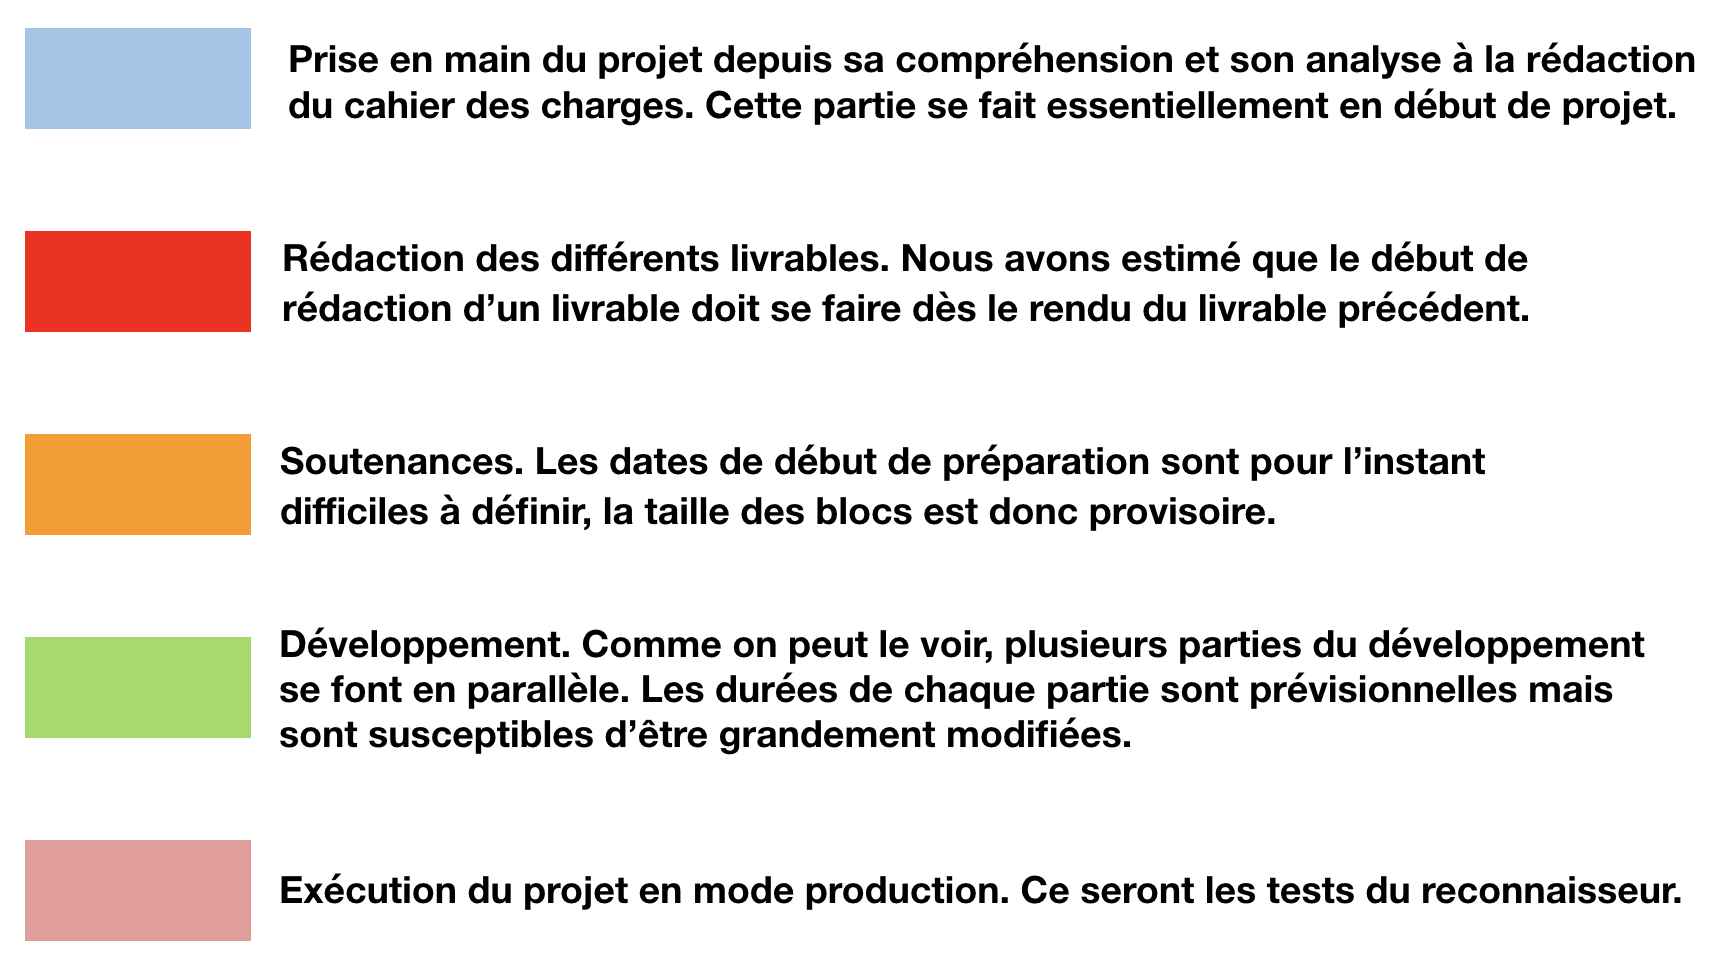
\includegraphics[width=\linewidth]{legende.png}
\end{center}
\end{mdframed}